\chapter{Lorem Ipsum yet again}
\label{sec:Lorem_Ipsum_yet_again__chapter_one}

Lorem ipsum dolor sit amet, consectetur adipiscing elit. Sed nec aliquam justo, eget efficitur neque. \textbf{Nam dignissim semper dignissim}. Etiam at aliquet massa. Aenean tempor augue sed justo bibendum gravida. In ex velit, fermentum sit amet sapien ut, egestas facilisis velit. Nulla nec pulvinar massa. Aenean mattis ipsum vitae augue porta accumsan. Vestibulum sit amet aliquam elit, rutrum mattis nulla (\autoref{sec:The_benefits_of_being_surrounded_by_animals__chapter_two}).

\section{Humans are cats' pets, in Lorem Ipsum}
\label{sec:Humans_are_cats'_pets,_in_Lorem_Ipsum__chapter_one}
Donec eget imperdiet nisl. Vestibulum scelerisque venenatis ante, eu varius tortor bibendum ut. In pretium varius tempus. Praesent posuere rhoncus porttitor. Pellentesque lobortis turpis leo, ut ultricies velit volutpat sit amet (\autoref{fig:a_cat_being_pet}). Donec consequat rutrum nisl, ac porttitor orci fringilla id. Curabitur fermentum facilisis interdum. Nunc hendrerit nec leo sit amet fermentum. Vivamus tempus suscipit libero at porttitor.

\begin{figure}[H]
	\centering
	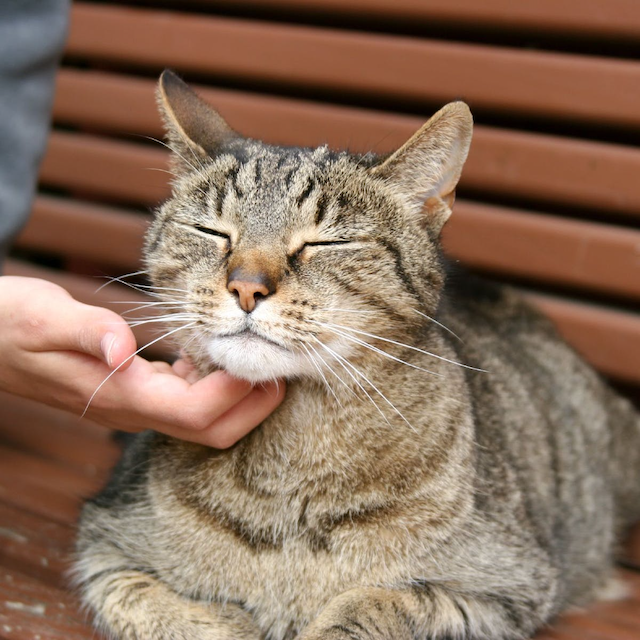
\includegraphics[width=0.4\linewidth]{Figures/cat.png}
	\caption{Here is a clear example of the submissiveness of "owners" to their "pets". The reverse paradigm explains this better.
}
	\label{fig:a_cat_being_pet}
\end{figure}

In commodo luctus sapien, quis lacinia ante faucibus a. Maecenas placerat efficitur gravida. Praesent in sem sed massa hendrerit vestibulum in sit amet nisi. Maecenas elementum nulla dui, sit amet malesuada ligula facilisis eget. Duis lacinia dolor ut purus mollis, ut dignissim diam lacinia. Nullam \footnote{ This is not meant in a strict sense, but rather as an intuitive analogy.
} cursus, orci sed aliquet porttitor, purus ante vulputate eros, a porttitor elit mauris sed ante. Proin eu lacus augue. In hac habitasse platea dictumst. Integer et lectus a nunc dictum rhoncus ac ut enim \autoref{eq:one_plus_one}. Mauris mattis lectus nec volutpat sodales (\autoref{sec:Historical_evidence__chapter_one}). Etiam in placerat quam. Sed tellus lectus, elementum et est ac, tincidunt dignissim risus. Maecenas eu erat sit amet arcu efficitur porta eget non elit \cite{Feline1999, Smooth2010}.

\begin{equation}
\label{eq:one_plus_one}
y = 1 + 1
\end{equation}

Nulla aliquam sapien nunc, ut ornare urna dignissim feugiat \hl{external note}. Maecenas ac leo nunc. Vestibulum nec eleifend est. Aenean at euismod purus. Aenean sagittis mauris maximus ultricies molestie. Aliquam fringilla diam venenatis odio interdum, vel iaculis neque scelerisque. Quisque eu ante odio. Proin aliquet nunc nisi, eleifend aliquam odio volutpat vel. Aliquam sagittis fringilla lectus, vitae auctor arcu elementum et. 


\section{Historical evidence}
\label{sec:Historical_evidence__chapter_one}
Quisque bibendum malesuada erat, nec auctor nisi dapibus vel. Maecenas ut lectus iaculis, laoreet lacus faucibus, fermentum purus. Etiam diam nibh, iaculis ac est sed, tincidunt vulputate urna. Duis malesuada suscipit dui at vestibulum. Proin laoreet purus in purus molestie fermentum.

\begin{displayquote}
 Nulla aliquam sapien nunc, \hl{ut ornare urna dignissim feugiat}. Maecenas ac leo nunc. Vestibulum nec eleifend est. Aenean at euismod purus. Aenean sagittis mauris maximus ultricies molestie. Aliquam fringilla diam venenatis odio interdum, vel iaculis neque scelerisque. Quisque eu ante odio.
\end{displayquote}

